% !TeX spellcheck = en_GB
%%=============================================================================
%% Methodologie
%%=============================================================================
% TODO Nakijken
\chapter{\IfLanguageName{dutch}{Methodologie}{Methodology}}
\label{ch:methodologie}
% Hoe ben je te werk gegaan? Verdeel je onderzoek in grote fasen, en licht in elke fase toe welke stappen je gevolgd hebt. Verantwoord waarom je op deze manier te werk gegaan bent. Je moet kunnen aantonen dat je de best mogelijke manier toegepast hebt om een antwoord te vinden op de onderzoeksvraag.

In this chapter the migration from Windows Server 2016 to Windows Server 2019 will be researched. This migration will first be performed using the in-place migration method. Microsoft heavily focused on the improvement for this form of migration. This should make it more resilient and safer to use. Afterwards the process will be repeated using a system migration. After this the migration of a typical SAP environment, as described by Delaware, from Windows Server 2016 to Windows Server 2019 will be examined. To continue the different versions of the container images will be analysed. How these can lower virtual machine overhead, and improve virtualization efficiency will be reviewed. Finally, their will be a discussion about how the new features that come with Windows Server 2019 can be leveraged in the migrated infrastructure. But first the infrastructure that was used for this proof of concept will be discussed.

\section{Technical specifications of the proof of concept setup}
The proof of concept was made on a bare-metal server running Windows Server 2016. The proof of concept environment was than virtualized using Hyper-V. 
\begin{itemize}
	\item CPU: Intel Xeon E5620
	\item RAM: 96 GB 
	\item HDD: 500 GB
	\item OS Version: Windows Server 2016
	\item Hyper-V role installed
	\item Administrative rights on the device
\end{itemize}
The proof of concept environment was based on the Modern Desktop Deployment and Management Lab Kit provided by Microsoft. \autocite{Gallagher2018}
This to make replication of the environment simple and efficient.
\\
The Modern Desktop Deployment and Management Lab Kit consists of the components in Table \ref{tab:MDDMLK2016}.
\\

\begin{table}[ht]
	\centering
	\begin{adjustbox}{width=1\textwidth}
	\begin{tabular}{l|l}
		Server Name  & Roles \& Products                                                  	 \\ 
		\hline
		HYD-DC1      & Active Directory Domain Controller, DNS, DHCP, Certificate Services 	   \\
		HYD-MDT1     & Microsoft Deployment Toolkit                                        		\\
		& Windows 10 1809 ADK                                                 					 \\
		& Windows Deployment Services                                         					  \\
		HYD-CM1      & System Center Configuration Manager 1806                            		   \\
		& Windows Deployment Services                                         						\\
		& Microsoft Deployment Toolkit                                         						 \\
		& Windows 10 1809 ADK                                                 			 			  \\
		& Windows Software Update Services                                        		  			   \\
		& Microsoft SQL Server 2014                                           						    \\
		HYD-APP1     & Microsoft BitLocker Administration and Monitoring                   				 \\
		& Microsoft SQL Server 2014                                          							  \\
		HYD-GW1      & Remote Access for Internet Connectivity                           				   \\
		HYD-INET1    & Simulated Internet                                                			 	    \\
		HYD-VPN1     & Remote Access for VPN                                             				     \\
		HYD-CLIENT1  & Windows 10 1809 Domain Joined                                  					      \\
		& Office 365 ProPlus Build 16.0.11121.20000                         								   \\
		HYD-CLIENT2  & Windows 10 1809 Domain Joined                                     					    \\
		& Office 365 ProPlus Build 16.0.11121.20000                           									 \\
		HYD-CLIENT3  & Windows 10 1809 Workgroup                                         						  \\
		HYD-CLIENT4  & Windows 10 1809 Workgroup                                          						   \\
		HYD-CLIENT5 & Bare metal (no installations)                                      						    \\
		HYD-CLIENT6 & Bare metal (no installations)                                       							 \\
		HYD-CLIENT7  & Windows 7 Domain Joined                                            
	\end{tabular}
	\end{adjustbox}
	\caption[Lab Kit Components]{Modern Desktop Deployment and Management Lab Kit Components}
	\scriptsize	
	Adapted from \cite{MicrosoftCorporation2019}
	\label{tab:MDDMLK2016}
\end{table}

	
Only HYD-CLIENT1 will be kept in the environment. Connection to the other \acrshort{vm}s can be made using the credentials in Table \ref{tab:MDDMLKC2016}.
\begin{table}[ht]
	\centering
	\begin{adjustbox}{width=1\textwidth}
	\begin{tabular}{l|lll}
		User                 & Access Type              & User Name                    & Password \\
		\hline
		Local Administrator  & Administrative           & Administrator                & P@ssw0rd \\
		Domain Administrator & Enterprise Administrator & CORP\textbackslash{}LabAdmin & P@ssw0rd
	\end{tabular}
	\end{adjustbox}
	\caption[Lab Kit Credentials]{Modern Desktop Deployment and Management Lab Kit Credentials}
	\scriptsize	
	Adapted from \cite{MicrosoftCorporation2019}
	\label{tab:MDDMLKC2016}
\end{table}
\\
Additionally Windows Admin Center will be installed on the gateway server HYD-GW1. 
\section{Upgrading the \acrshort{os}}
\subsection{In-place migration to Windows Server 2019}
In this subsection an in-place migration will be performed on the \acrfull{dc} from Windows Server 2016 to Windows Server 2019. To continue the operation of the applications running on the \acrshort{dc} and the connections to the other servers in the domain will be verified. Possible problems and solutions will be discussed as they reveal themself.
\subsubsection{Prerequisites}
Before starting the migration, it is important to verify that the server is backed-up. Be sure to check when the last back-up was performed and if one has ever been successfully restored. After this it is important to verify that all the third-party applications on the server are supported by the newest version of the \acrshort{os}. Finally, the forest and domain need to be prepared for the migration. The installation media provides tools for this. The following code completes this process, as is shown in Figure \ref{fig:inplace1}. Be sure to verify the mounting point of the installation media, in this scenario it has been mounted to D:\textbackslash .

\begin{lstlisting}[breaklines]
:d
cd support\adprep
adprep /forestprep
adprep /domainprep
\end{lstlisting}
\begin{figure}[h]
	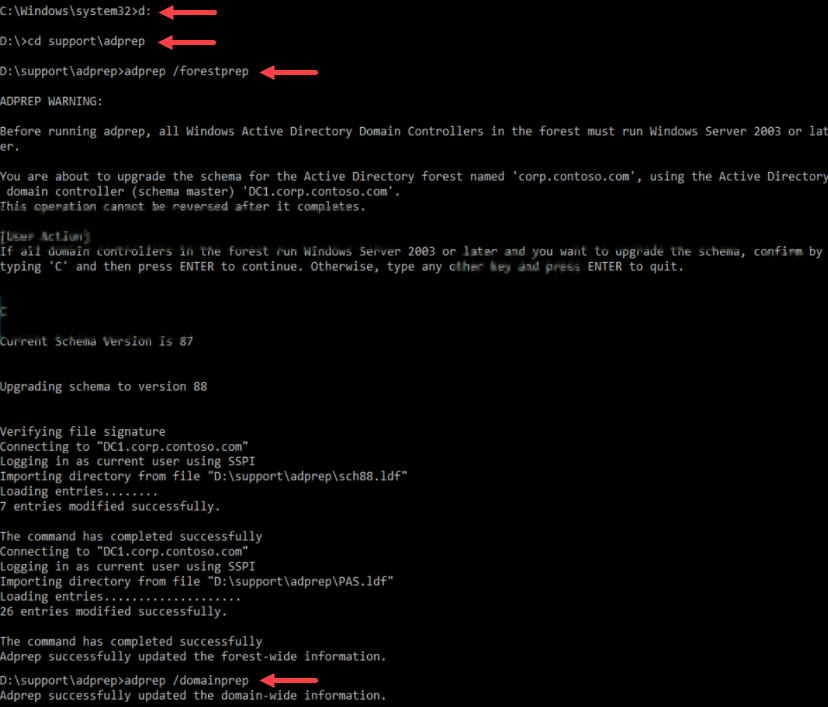
\includegraphics[height=8cm]{img/In-Place_WS_1.png}
	\captionsetup{width=0.8\linewidth}
	\centering		
	\caption{Preparing the forest and domain}
	\label{fig:inplace1}
\end{figure}

\subsubsection{In-place migration}
After the previous step the setup from the installation is to be launched. From this point on the migration process has been visualized in Figure \ref{fig:inplace}. If there is no figure present of the current screen it is expected to click next and continue the in-place migration. Be sure to not use the evaluation version of Windows Server 2019, since this does not support in-place migrations.
\begin{figure}[h]
	\begin{subfigure}{0.5\textwidth}
		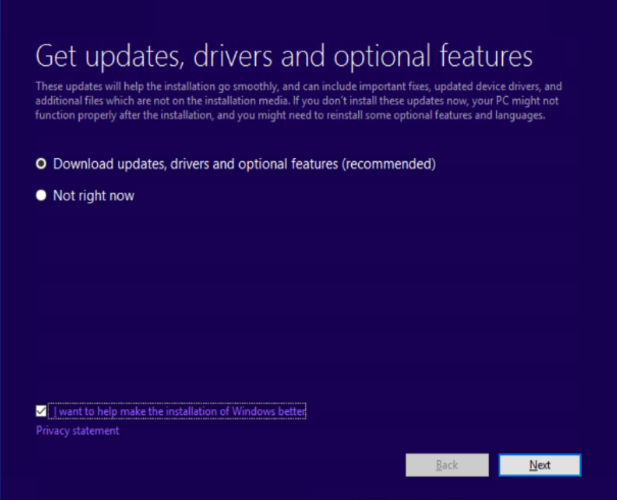
\includegraphics[width=0.9\linewidth,height=4.3cm]{img/In-Place_WS_2.png}
		\captionsetup{width=0.8\linewidth}
		\centering		
		\caption{Click next to migrate}
		\label{fig:inplace2}
	\end{subfigure}
	\begin{subfigure}{0.5\textwidth}
		\captionsetup{width=0.8\linewidth}
		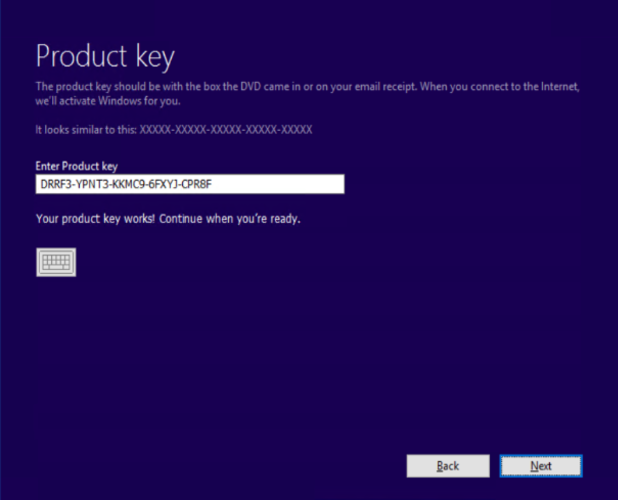
\includegraphics[width=0.9\linewidth,height=4.3cm]{img/In-Place_WS_3.png}
		\centering
		\caption{Enter the product key}
		\label{fig:inplace3}
	\end{subfigure}
\end{figure}
\begin{figure}[h]\ContinuedFloat
	\begin{subfigure}{0.5\textwidth}
		\captionsetup{width=0.8\linewidth}
		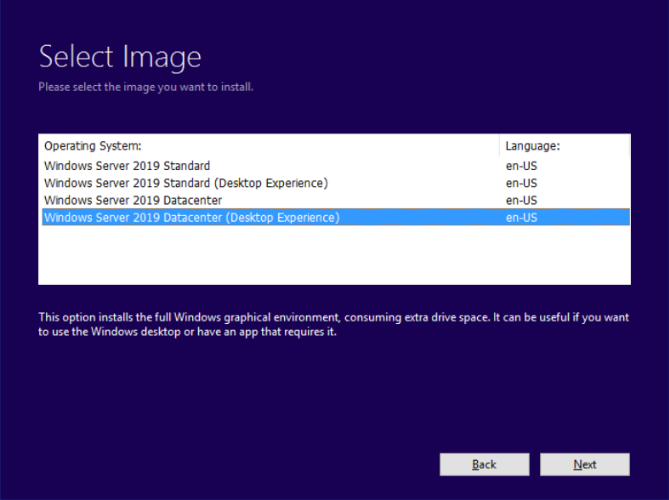
\includegraphics[width=0.9\linewidth,height=4.3cm]{img/In-Place_WS_4.png} 
		\centering
		\caption{Select a version of choice}
		\label{fig:inplace4}
	\end{subfigure}
	\begin{subfigure}{0.5\textwidth}
		\captionsetup{width=0.8\linewidth}
		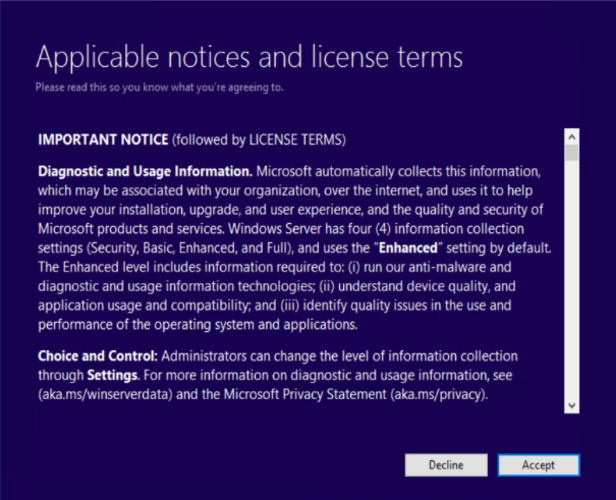
\includegraphics[width=0.9\linewidth,height=4.3cm]{img/In-Place_WS_5.png}
		\centering
		\caption{Accept the licence terms}
		\label{fig:inplace5}
	\end{subfigure}
\end{figure}
\begin{figure}[h]\ContinuedFloat
	\begin{subfigure}{0.5\textwidth}
		\captionsetup{width=0.8\linewidth}
		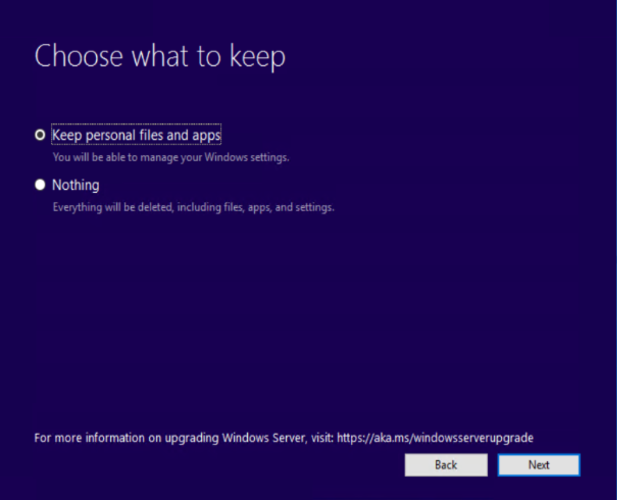
\includegraphics[width=0.9\linewidth,height=4.3cm]{img/In-Place_WS_6.png} 
		\centering
		\caption{Select "Keep personal files and apps" to perform an in-place migration}
		\label{fig:inplace6}
	\end{subfigure}
	\begin{subfigure}{0.5\textwidth}
		\captionsetup{width=0.8\linewidth}
		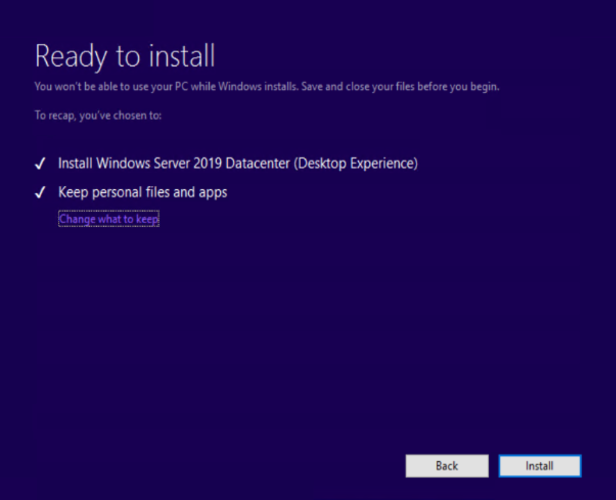
\includegraphics[width=0.9\linewidth,height=4.3cm]{img/In-Place_WS_7.png}
		\centering
		\caption{Review the settings and start the installation}
		\label{fig:inplace7}
	\end{subfigure}
	\caption{The in-place migration process}
	\label{fig:inplace}
\end{figure}
\subsubsection{Verification}
% nltest /sc_query:corp.contoso.com
\subsection{Migration to Windows Server 2019}
\subsubsection{Prerequisites}
\subsubsection{Migration}
\subsubsection{Verification}
\subsection{Conclusion}
% TODO Conlusion
% https://raw.githubusercontent.com/coreyp-at-msft/ws-upgrade-center/dev/en-US/media/upgrade-paths-2-small.png
% Explain how 2016 -> 2019 is easy but previous version can require consecutive migrations that each bring their own "bagage"
\section{SAP migration}
\subsection{Technical specifications of SAP environment}
\subsection{Migration of SAP}
\section{Windows, Windows Server Core and Nano Server}
In this final section a comparison shall be made between the Windows, Windows Server Core and Windows Nano Server container images. At first the advantages of the new versions of the images will be discussed. This involves a comparison between version 1709 of the and version 1809 of the base container images. This will consist of comparing the size of the base images and their performance. Afterwards the different use cases of the various versions will be discussed. These images have been tested in an environment as described in the following subsection.

\subsection{Technical specifications of the container environment}
The proof of concept environment for the Windows Server base container images was built using the Microsoft Azure platform. It uses the Standard D2s v3 (2 vcpus, 8 GB memory) Azure \acrshort{vm}, running the Windows Server 2019 Datacenter Server Core and Containers image.
The following packages will be installed inside the \acrshort{vm}:
\begin{itemize}
	\item Docker
	\item Hyper-V
	\item Windows Containers
	\item Chocolatey
	\item Git
\end{itemize}
The procedure to generate container environment is described in Appendix \ref{Containers_Azure}.

\subsection{The advantages of version 1809}
With the arrival of version 1809, the \acrfull{sac} equivalent of Windows Server 2019, their have been improvements to the base images. First of all, the overall size of the base images has been significantly reduced. This can be seen in Figure \ref{fig:container_size}. The only exception is the size of the Nano Server, which has slightly increased in comparison to its previous version. 
%TODO Why has Nano Server enlarged?
The size of the different base images has been obtained by downloading and expanding them as described below. This was done through Windows Powershell from inside the \acrshort{vm} that was previously created on the Azure platform. 

\begin{lstlisting}[breaklines]
docker image pull mcr.microsoft.com/windows:1809
docker image pull mcr.microsoft.com/windows/servercore:1809
docker image pull mcr.microsoft.com/windows/nanoserver:1809  
docker image pull mcr.microsoft.com/windows/servercore:1709 
docker image pull mcr.microsoft.com/windows/nanoserver:1709   
docker images | Out-File .container_images.csv
Import-Csv -Path .container_images.csv
\end{lstlisting}

\begin{figure}[h]
	\captionsetup{width=0.8\linewidth}
	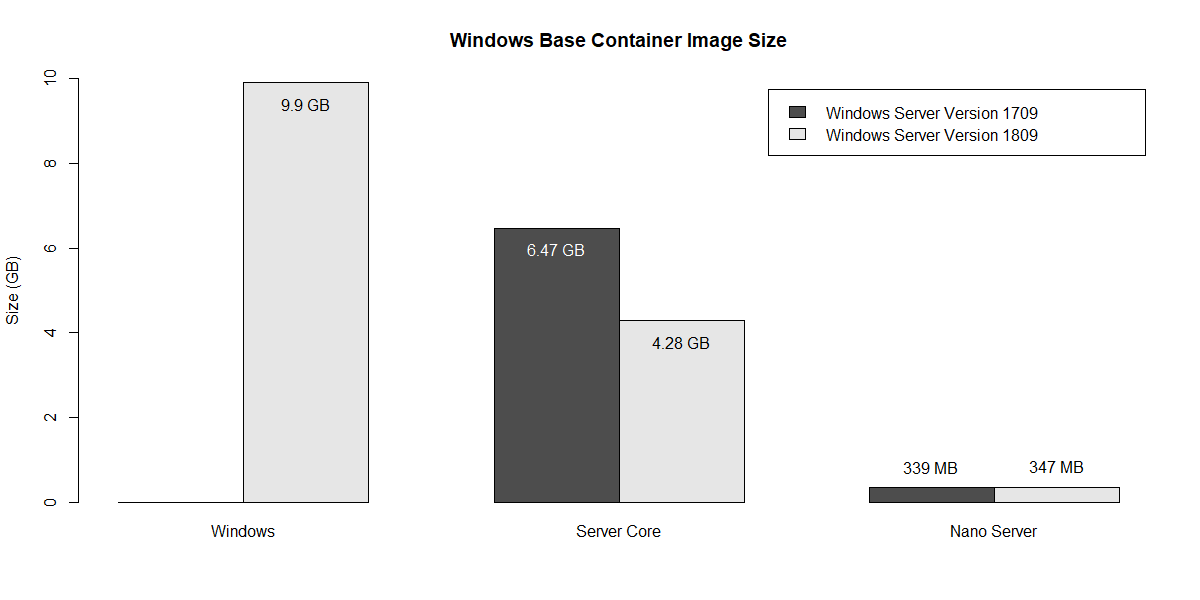
\includegraphics[width=0.9\linewidth]{img/Container_size.png}
	\centering
	\caption{Comparison of the Windows base container image size}
	\label{fig:container_size}	
\end{figure}

In this paragraph the performance of the images shall be tested. This will be done using \href{https://benchmarkdotnet.org/}{"BenchmarkDotNet"}, a .NET library made for benchmarking. \autocite{Akinshin2019} Benchmarking using this library is done by calculating \acrfull{md5} and \acrfull{sha} hash functions. The former is mostly used in the genereation of identifiers, as it is not deemed secure enough for data security. The latter is better suited for this, but has since been improved by \acrfull{sha3}. \autocite{Enkov2017}
\\
The container will be automatically built using a Dockerfile, each Dockerfile has its own corresponding base container image. This is needed to add the required packages inside the container to successfully perform the benchmark. For the Windows and Server Core image these get added manually, the Nano Server images were provided by Microsoft. Following commands need to be executed on the \acrshort{vm} that was created on the Azure platform to benchmark every container individually.
\begin{lstlisting}[breaklines]
git clone https://github.com/jensdufour/Benchmark.git
cd Benchmark	
docker build -t benchmark1 --isolation=hyperv -f .\WindowsNanoserver1709.dockerfile .
docker build -t benchmark2 --isolation=hyperv -f .\WindowsServercore1709.dockerfile .
docker build -t benchmark3 --isolation=hyperv -f .\WindowsNanoserver1809.dockerfile .
docker build -t benchmark4 --isolation=hyperv -f .\WindowsServercore1809.dockerfile .
docker build -t benchmark5 --isolation=hyperv -f .\Windows1809.dockerfile .
\end{lstlisting}

%TODO Inleiding eerste grafiek
The results of running the individual benchmarks have been visualized in Figure \ref{fig:MD5} for MD5 and in Figure \ref{fig:SHA} for SHA-256. The figures show the average results after running the benchmarks twenty times. In Appendix \ref{benchmarkdata}, all the data can be found, as well as the initial results after running the benchmarks ten times. Eventual outliers have been removed. 

\begin{figure}[h]
	\captionsetup{width=0.8\linewidth}
	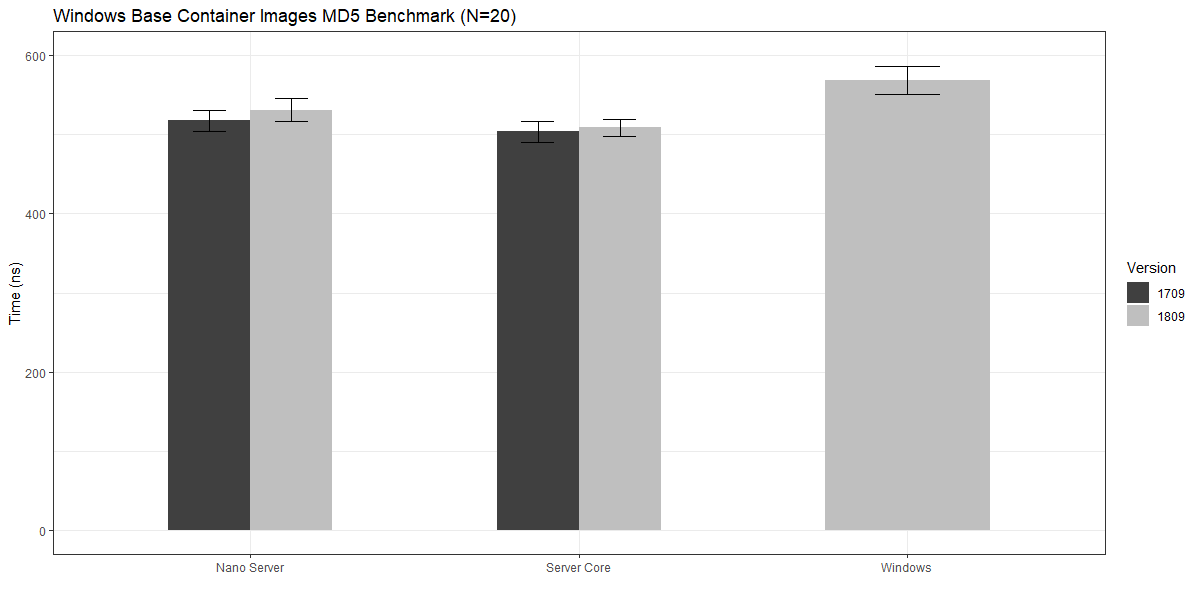
\includegraphics[width=0.9\linewidth]{img/MD5_20.png}
	\centering
	\caption{Windows Base Container Image MD5 Benchmark (N=20)}
	\label{fig:MD5}
\end{figure}

%TODO Inleiding tweede grafiek
Lorem ipsum dolor sit amet, consectetur adipiscing elit. Suspendisse porta, turpis at gravida ultrices, dolor lacus ornare ipsum, quis consectetur risus nunc ac lorem. Mauris fermentum elit non dictum feugiat. Nullam at metus ultricies, ultrices metus sit amet, hendrerit tortor. Lorem ipsum dolor sit amet, consectetur adipiscing elit. Suspendisse vehicula cursus nunc nec vestibulum. Orci varius natoque penatibus et magnis dis parturient montes, nascetur ridiculus mus. In ac faucibus purus, sed viverra turpis. Donec dolor massa, molestie ut eleifend id, porta quis nisl. Vivamus suscipit eu odio gravida euismod. Fusce nec lectus finibus, elementum nulla quis, ultricies magna.
Donec dolor massa, molestie ut eleifend id, porta quis nisl. Vivamus suscipit eu odio gravida euismod. Fusce nec lectus finibus, elementum nulla quis, ultricies magna.

\begin{figure}[h]
	\captionsetup{width=0.8\linewidth}
	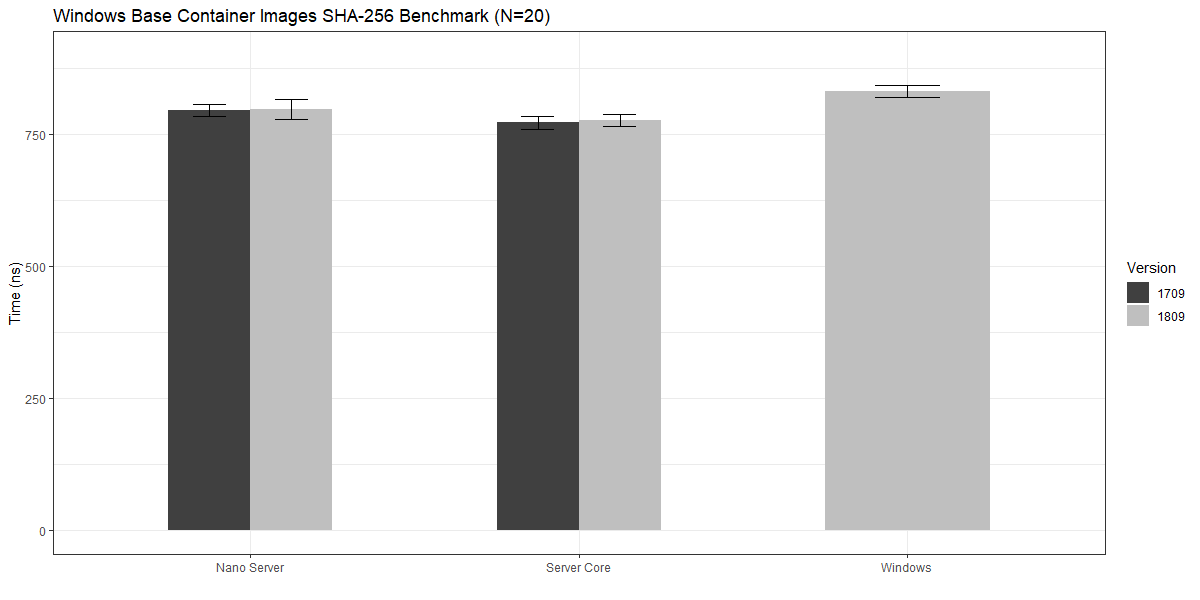
\includegraphics[width=0.9\linewidth]{img/SHA_20.png}
	\centering
	\caption{Windows Base Container Image SHA-256 Benchmark (N=20)}
	\label{fig:SHA}
\end{figure}

%TODO Conclusie herschrijven aan de hand van bovenstaande grafieken
 When looking at the result of the benchmarks of Server Core and Nano Server, it is clear that the performance of both versions is along the same lines. However, the overall reduction in size and the additional functions that have been added, as discussed in Chapter \ref{ch:stand-van-zaken}, make a strong case for the deployment of the latter. It is important to note that the kernel version of the \acrshort{os} must match the Windows image. While using Hyper-V isolation can circumvent this, it is not recommended since the additional virtualization of the kernel will lower the performance of the container. The latest of images also includes the Windows base container. This opens a whole array of new possibilities. The use case of this one, and the others, will be discussed in the following subsection.

\subsection{Usage of Windows, Windows Server Core and Windows Nano Server}
The smallest one that is offered is the Nano Server. This image is aimed at rapid and lightweight deployment using containers. It has been specifically designed for "born in the cloud" applications. This is a term that has multiple usages, it refers to applications that are not legacy products. Applications that provide an agile deployment and offer on-demand availability. It is in no way meant to run typical Windows services. The bigger brother of Nano Server, Server Core, is more suited for this. 
This image offers application compatibility and has a wide array of built-in Windows roles and features. On top of this it has full .NET Framework support instead of the basic .NET Core that is offered by the Nano Server. 
The final image that is offered is the new kid on the block. The Windows image offers almost all the Windows components in a lightweight package. This makes it exceptionally useful for the automation of workloads. 
\\
Thanks to the further development to these images their footprint has been reduced significantly. Although, older containers from Windows Server 2016 can still be run through Hyper-V isolation, it is recommended to rebuild them with the latest available images.




